\documentclass[twocolumn]{article}

%% ─── Packages ────────────────────────────────────────────────────────────────
% Core packages only — all present in BasicTeX
\usepackage[margin=1in]{geometry}
\usepackage{amsmath,amssymb}
\usepackage{booktabs}
\usepackage{array}
\usepackage{graphicx}
\usepackage{xcolor}
\usepackage{hyperref}
\usepackage{microtype}

\hypersetup{
  colorlinks=true,
  linkcolor=blue!70!black,
  citecolor=blue!70!black,
  urlcolor=blue!70!black,
}

%% ─── Title ───────────────────────────────────────────────────────────────────
\title{%
  \textbf{KB: A Facts-First Codebase Knowledge System with\\
  Multi-Objective Exploration Loss Evaluation}%
}

\author{%
  Jacob Rosenzweig \\
  \textit{Independent Research} \\
  \texttt{rosenjcb@gmail.com}
}

\date{June 2026}

%% ─── Document ────────────────────────────────────────────────────────────────
\begin{document}

\maketitle

%% ─── Abstract ────────────────────────────────────────────────────────────────
\begin{abstract}
LLM-based developer agents suffer from two compounding inefficiencies: each
session begins with an empty context window, forcing costly re-exploration of
the codebase, and current evaluation frameworks measure only whether the final
answer is correct, hiding the exploration cost that produced it.  We present
two complementary contributions.

\textbf{KB} is a local-first, facts-first codebase knowledge system that
converts knowledge maintenance into a side-effect of normal development work.
KB indexes source code deterministically via AST analysis (tree-sitter) and
documentation via sentence-level fact extraction, storing atomic facts in a
SQLite graph with typed edges.  At query time, a multi-pond BFS loop merges
lexical (BM25/FTS5), semantic (embedding), and graph-walk evidence streams into
a ranked fact pool, exiting on a scored sufficiency condition.

\textbf{MOEL} (Multi-Objective Exploration Loss) is a quantitative evaluation
framework that measures agent efficiency under three controlled conditions:
Condition N (raw filesystem baseline), Condition K (KB-equipped), and Condition
O (oracle context injection).  MOEL combines three normalized loss terms—LLM
jury semantic loss ($L_\text{jury}$), trajectory inefficiency
($L_\text{trajectory}$), and resource consumption ($L_\text{resource}$)—into a
single weighted scalar $L_\text{MOEL}$.  Bias mitigation (position debiasing,
verbosity normalization, self-enhancement down-weighting, family diversity
enforcement) and statistical calibration via per-judge logistic regression are
built in.

The headline metric is a budget-normalized success score
$S = 0.60\,Q + 0.30\,E_{\text{tok}} + 0.10\,E_{\text{speed}}$ that blends answer
quality with token economy and latency, scored identically for KB-equipped and
control runs so the two are directly comparable.  Empirically, KB reaches a
quality component $Q = 0.86$ and pass rate $1.00$ on the KB self-check suite
(evidence handling 4.00/4.00) and $Q = 0.92$, pass rate $0.75$ on the external
raylib C library benchmark (correctness 3.88/4.00, evidence handling
3.88/4.00).  All MOEL framework components are fully implemented and
unit-tested, with benchmark alignment against SWE Atlas, SWE-ContextBench, and
CodeScaleBench established.
\end{abstract}

%% ─── Body ────────────────────────────────────────────────────────────────────
%% ─── Introduction ───────────────────────────────────────────────────────────
\section{Introduction}
\label{sec:intro}

Large language models (LLMs) have dramatically changed how developers interact
with codebases, enabling agents to autonomously resolve real-world software
engineering issues~\cite{yang2024sweagent}.  Yet the dominant interaction model remains \emph{ephemeral}:
each agent session begins with an empty context window, forcing the model to
re-discover facts about the codebase from scratch.  This creates a compounding
inefficiency—teams that rely on LLM assistants must accept that every question
triggers a fresh, expensive, and error-prone tour of the filesystem.

Two failure modes characterize this status quo.  First, \textbf{exploration
waste}: agents read far more source files than necessary before reaching an
answer, because there is no prior accumulation of structured knowledge to query.
On representative SWE-Bench tasks, text-based agents spend up to 21 steps
navigating via grep and line-range reads to locate a single target function---work
that structured pre-indexed facts resolve in two or three
queries~\cite{kim2025codestruct}.  Second,
\textbf{context dilution}: irrelevant context degrades LLM
reasoning~\cite{shi2023distracted}, and brittle
string-matching edits fail when whitespace or formatting drifts~\cite{kim2025codestruct}.

Existing retrieval-augmented generation (RAG) systems~\cite{lewis2020rag}
address the first problem partially, but are designed for static document
corpora, not living codebases with interleaved code, documentation, and
decision history.  Code-search benchmarks such as
CodeSearchNet~\cite{husain2019codesearchnet} evaluate individual retrieval
steps in isolation, ignoring the sequential cost of multi-step agent
exploration.

We present \textbf{KB}, a local-first, \emph{facts-first} codebase knowledge
system that:
\begin{enumerate}
  \item[(1)] indexes a repository's code and documentation into a persistent
    SQLite store of atomic, citable facts via deterministic AST analysis and
    sentence-level fact extraction;
  \item[(2)] exposes those facts to LLM agents through a multi-pond BFS
    retrieval loop that merges lexical (BM25), semantic (embedding), and
    graph-walk evidence streams without manual query engineering.
\end{enumerate}

Critically, KB's value is only as compelling as the evidence that it actually
reduces agent exploration cost.  Rubric-based Q\&A scoring—the standard in
prior agent evaluation—captures answer quality but is blind to \emph{how} the
agent arrived at that answer.  A system that reads 40 files before synthesizing
a correct response and one that queries two facts look identical under a
pass/fail quality signal.

To fill this gap, we introduce the \textbf{Multi-Objective Exploration Loss
(MOEL)} evaluation framework.  The harvest runner scores both KB (K) and a
real-agent control (N) on the same eight questions and reports the headline
grade $\Delta S = S_K - S_N$ (Eq.~\ref{eq:delta-s}).  A complementary deep
pipeline runs tasks under three conditions (N, K, O) and aggregates exploration
loss into $L_\text{MOEL}$.

Figure~\ref{fig:system-overview} illustrates the end-to-end system.  Our
contributions are:

\begin{enumerate}
  \item \textbf{KB}: a facts-first codebase knowledge system with deterministic
    AST indexing and a multi-pond hybrid retrieval orchestrator.

  \item \textbf{MOEL}: a multi-objective evaluation framework comprising three
    normalized loss functions ($L_\text{jury}$, $L_\text{trajectory}$,
    $L_\text{resource}$), bias-mitigated LLM jury scoring, and
    logistic-regression calibration on a 20-sample human-annotated set.

  \item \textbf{Empirical results}: build-under-test evaluation compares the
    main and optimized KB binaries against fixed \texttt{kb} and \texttt{raylib}
    repository snapshots.  The optimized build preserves pass rate on both
    targets and keeps fact/document counts stable (Table~\ref{tab:latest-quality}).
    Fresh K-vs-control $\Delta S$ rows are pending because \LatestControlStatus{}.
\end{enumerate}

%% ─── Figure: System Overview placeholder ─────────────────────────────────────
\begin{figure}[t]
\centering
\fbox{
  \parbox{0.92\columnwidth}{
    \centering
    \vspace{0.4cm}
    \textit{\textbf{[FIGURE 1 — System Overview]}} \\[6pt]
    A three-panel horizontal flow diagram: \\
    \textbf{Left panel} — Developer working directory with source files,
      markdown, and git history feeding into \texttt{kb init} (AST indexer +
      sentence segmenter + fact extractor). \\
    \textbf{Center panel} — SQLite knowledge store: \texttt{facts} table
      (doc + code facts), \texttt{fact\_edges} graph, \texttt{fact\_embeddings}
      semantic index, \texttt{documents} (human-readable artifacts). \\
    \textbf{Right panel} — LLM agent loop: \texttt{kb query} dispatches
      multi-pond BFS retrieval, passes ranked facts to LLM, returns grounded
      prose answer. \\
    Below all panels: harvest runner reporting $\Delta S = S_K - S_N$ (K vs.\ real
      agent); deep MOEL harness (N/K/O toy-tool conditions) reporting
      $L_\text{MOEL}$.
    \vspace{0.4cm}
  }
}
\caption{End-to-end KB system.  Primary harvest grade: $\Delta S$ (K vs.\ real
agent); deep MOEL harness adds $L_\text{MOEL}$ under toy-tool N/K/O conditions.}
\label{fig:system-overview}
\end{figure}

%% ─── Related Work ────────────────────────────────────────────────────────────
\section{Related Work}
\label{sec:related}

\subsection{LLM-Based Code Agents and Tools}

SWE-Agent~\cite{yang2024sweagent} and Agentless~\cite{xia2024agentless} are
representative systems in which agents navigate repositories through file-read
and string-edit operations.  AutoCodeRover~\cite{zhang2024autocoderover}
augments this with symbol indices and file maps to guide localization.
CODESTRUCT~\cite{kim2025codestruct} replaces text-based edits with AST-grounded
primitives (\texttt{readCode}/\texttt{editCode}), reducing input tokens by
12--38\% and improving SWE-Bench Verified Pass@1 by up to 5.0pp.  KB is
complementary to these systems: whereas CODESTRUCT improves the \emph{action
interface} once a target is located, KB improves \emph{context retrieval} by
replacing filesystem exploration with structured fact lookup.  The two
approaches can be composed.

\subsection{Retrieval-Augmented Generation}

RAG~\cite{lewis2020rag} grounds LLM answers in retrieved passages, but standard
RAG pipelines are designed for static document collections.  They do not model
the inter-entity relationships that characterize codebases (function calls,
class hierarchies, module imports), and they treat retrieval as a one-shot
lookup rather than an adaptive loop.  KB's multi-pond BFS loop merges five
evidence streams per pass and exits on a scored sufficiency condition, making
retrieval quality a function of graph density rather than fixed index size.

\subsection{LLM Evaluation Frameworks}

Evaluating LLM outputs with another LLM (LLM-as-judge) is established in
MT-Bench~\cite{zheng2023judging} and AlpacaFarm~\cite{dubois2024alpacafarm}.
Known failure modes include position bias, verbosity bias, and self-enhancement
bias.  PandaLM~\cite{wang2023pandalm} trains a dedicated judge model to
mitigate these.  MOEL's jury module addresses the same biases at inference time
through position debiasing (swapped-order consistency), verbosity normalization
($\log_{1+}$ length scaling), self-enhancement down-weighting ($\times 0.5$ for
same-family judges), and family diversity enforcement---without requiring a
fine-tuned judge.  Unlike prior work, MOEL is not outcome-only: it combines
the LLM jury with an AST-structural loss and trajectory/resource losses so that
efficiency failures are numerically visible.

\subsection{Agent Efficiency Measurement}

SWE-ContextBench measures token cost and cache efficiency across context
injection strategies; CodeScaleBench evaluates tool validity across repository
scale classes.  Neither framework provides a unified scalar loss that spans
correctness, trajectory, and resource consumption simultaneously.  The closest
prior work is SWE-Atlas, which verifies agent-declared file manifests against
live \texttt{git diff} output.  MOEL's \texttt{ManifestValidator} adopts the
same live-diff approach and extends it with a \texttt{MutationValidator} that
applies tree-sitter AST body stubs to confirm causal linkage between agent
changes and test coverage.

\subsection{AST-Based Code Analysis}

Tree-sitter~\cite{falleri2014gumtree} and related tools provide fine-grained
AST differencing.  ASTNN~\cite{alon2019code2vec} uses AST path embeddings for
code representation learning.  MOEL's $L_\text{AST}$ adopts a simpler but
interpretable measure: Jaccard distance over named exported declarations,
computed deterministically without learned components, making it reproducible
across model versions.

%% ─── System: KB ──────────────────────────────────────────────────────────────
\section{KB: A Hybrid-Retrieval Codebase Knowledge System}
\label{sec:system}

\subsection{Knowledge Representation}

KB represents a codebase as three kinds of independently retrievable
\emph{units} stored in a SQLite database, rather than as a single graph of
atomic facts:
\begin{itemize}
  \item \textbf{Documents} --- whole markdown files (README, docs) stored
    verbatim in a \texttt{documents} table (\texttt{title}, \texttt{body},
    \texttt{content\_hash}, origin \texttt{git\_repo}); the retrieval unit is the
    entire document, not a sentence chunk.
  \item \textbf{Code symbols} --- exported declarations (functions, classes,
    interfaces, type aliases, constants) extracted by AST analysis and stored in
    a \texttt{code\_symbols} table with their name, \texttt{kind}, and source
    text.
  \item \textbf{Facts} --- curated natural-language claims in a \texttt{facts}
    table, retained for authoring provenance and as a third retrieval lane.
\end{itemize}

Each unit type has a paired FTS5 full-text index
(\texttt{documents\_fts}, \texttt{code\_symbols\_fts}, \texttt{facts\_fts}) and
an optional per-unit embedding vector (\texttt{doc\_embeddings},
\texttt{code\_embeddings}, and fact embeddings).  Documents and symbols are
associated through a flat \texttt{doc\_code\_links} table---a document is linked
to the symbols it describes.  This is deliberately \emph{not} a traversable
graph: there are no typed fact edges and no multi-hop neighborhoods.  An earlier
version of KB stored sentence-level facts in a \texttt{fact\_edges} graph and
walked it at query time; that graph was removed in favor of the flat,
depth-1 link table because unbounded neighborhood expansion made retrieval cost
scale with index connectivity rather than with the query.

\subsection{Indexing Pipeline}

\texttt{kb init} executes a fully deterministic indexing pipeline.
No LLM is invoked and no API cost is incurred.

\medskip
\noindent\textbf{Code symbols.}  For each source file, KB
invokes the \texttt{web-tree-sitter} WASM runtime with per-language export
queries to extract named declarations.  Each exported symbol becomes a
\texttt{code\_symbols} row keyed by \texttt{(git\_repo, rel\_path, name)}, storing
its kind and source text for later display and neural scoring.

\medskip
\noindent\textbf{Documents.}  Human-readable sources (README files, markdown
documentation) are ingested \emph{whole}: each file becomes one
\texttt{documents} row with a content hash for incremental re-indexing.  Open
Knowledge Format frontmatter is stripped so metadata never pollutes the body.
KB then records \texttt{doc\_code\_links} between a document and the symbols it
references.

\medskip
\noindent\textbf{Embeddings.}  After indexing completes, \texttt{kb init} runs a
best-effort embedding pass over documents and symbols: by default a local
on-device sentence-transformer (\texttt{all-MiniLM-L6-v2}); set
\texttt{KB\_EMBEDDER=gemini} to opt into hosted Gemini embeddings.  When no
embedder is available, rows keep a deterministic hash vector and neural scoring
degrades gracefully---init never blocks on embedding failure, and the lexical
lanes carry retrieval on their own.

The raylib snapshot in Table~\ref{tab:harvest-results}
(\RaylibKEntities{} entities, \RaylibKRels{} links)
completes init+scan in minutes on a laptop with no LLM indexing cost.

%% ─── Figure: KB Architecture (auto-rendered from figures/kb-arch.mmd) ─────────
\begin{figure}[t]
\centering
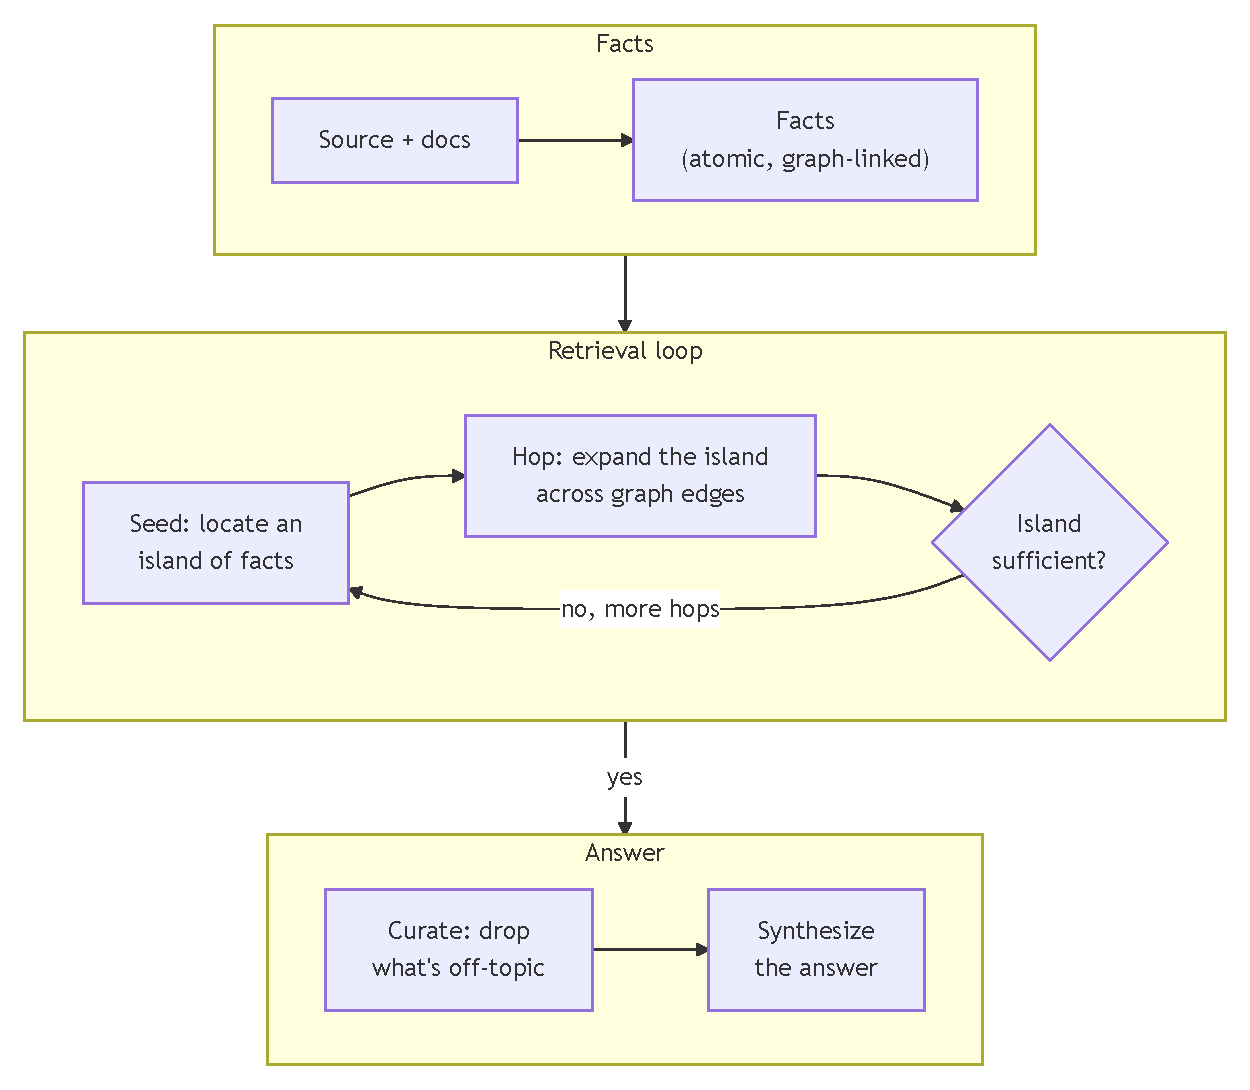
\includegraphics[width=\columnwidth]{figures/kb-arch.pdf}
\caption{KB indexing (top) feeds the hybrid retriever: six lexical/neural lanes over documents, symbols, and facts are fused by Reciprocal Rank Fusion, a depth-1 doc$\leftrightarrow$symbol hop enriches the pool, and a curator prunes before one-shot synthesis (bottom).}
\label{fig:kb-arch}
\end{figure}

\subsection{Retrieval: Hybrid Rank Fusion}
\label{subsec:retrieval}

At query time, KB runs a single-pass \emph{hybrid} retriever over the three unit
types.  For a query $q$ it opens six ranked lanes---each of
\{documents, code symbols, facts\} searched both lexically (BM25~\cite{robertson2009bm25}
over FTS5) and neurally (embedding cosine).  To avoid a full-table embedding scan
per query, the neural lanes re-rank the candidate pool that the lexical lanes
surfaced rather than scoring every vector in the index.

\medskip
\noindent\textbf{Reciprocal Rank Fusion.}  The six lists are combined with
Reciprocal Rank Fusion (RRF)~\cite{cormack2009rrf}: a unit at rank $i$ in a lane
contributes $1/(k + i)$ to its fused score, with damping $k = 60$.  RRF needs no
per-lane score calibration---it consumes only ranks---so lexical BM25 scores and
cosine similarities combine without a tuned weighting between them, and a unit
surfaced by several lanes accrues their contributions.

\medskip
\noindent\textbf{Depth-1 enrichment hop.}  After fusion, KB takes the top few
documents and symbols and follows \texttt{doc\_code\_links} exactly one hop: the
code a top document describes, and the documentation that describes a top symbol.
Hopped units enter \emph{below} every directly matched unit, so they enrich the
pool without displacing direct hits.  Because the link table is flat and the hop
is depth-1 by construction, retrieval cost is bounded by the candidate pool, not
by how densely the index is connected---the property the removed graph walk
lacked.  The top $\sim\!40$ fused units are handed to curation and synthesis.

\subsection{Post-Retrieval Curation}
\label{subsec:curation}

Rank fusion and the enrichment hop are deliberately \emph{broad}: they surface
units adjacent to, but not always directly about, the user's question.  When the
ranked pool is large enough, a \textbf{curator} runs \emph{before} synthesis.
It is judge-in-the-loop, not a static score floor:
\begin{enumerate}
  \item \textbf{Deterministic auto-keep}: units whose token overlap with the
    \emph{raw user question} exceeds a fixed threshold bypass the LLM (no cost,
    stable anchors).
  \item \textbf{Candidate cap}: only the top-ranked units enter the LLM verdict;
    the tail is dropped deterministically so large pools cannot overflow the
    structured keep/drop JSON.
  \item \textbf{Structured relevance verdict}: remaining candidates are sent to a
    single LLM call returning a structured verdict with \emph{keep} ids,
    \emph{gap} descriptions, and a \emph{sufficient} flag.
  \item \textbf{Drop}: every unit not in the keep set (except auto-kept rows) is
    removed from the synthesis context; there is no minimum keep fraction.
  \item \textbf{Gap re-discovery}: when the judge reports gaps and the set is not
    yet sufficient, the curator issues bounded hybrid searches per gap (excluding
    already-seen ids), merges new hits, and re-judges for up to a small round cap.
\end{enumerate}

On LLM or parse failure the curator \emph{fails safe} to the incoming pool for
small sets, and caps at the top-ranked subset for larger pools rather than
passing an unfiltered pool into synthesis.  Curator audit counts (kept, dropped,
re-queried) are recorded separately from the synthesis context for later
analysis---never injected back into the prompt as evidence.

\subsection{Answer synthesis}
\label{subsec:synthesis}

After retrieval and optional curation, \texttt{kb query} performs \emph{one-shot}
synthesis: a single LLM call over the curator-kept units (document bodies are
truncated to a per-unit character cap).  The synthesis prompt instructs
\emph{plain prose}: no inline ``(fact~$n$)'' citations and no trailing
Sources/Citations block; provenance is surfaced in a separate structured
evidence summary.  This is the path evaluated against the control agent in
\S\ref{subsec:results}---no multi-turn retrieval loop, matching how an external
agent would call KB for a standalone question.

%% ─── MOEL ─────────────────────────────────────────────────────────────────────
\section{MOEL: Multi-Objective Exploration Loss}
\label{sec:moel}

\subsection{Motivation}

Standard evaluation of LLM agents on code tasks measures whether the final
answer is correct.  This binary signal hides the cost of exploration: an agent
that issues 50 tool calls to reach a correct answer and one that issues 3 are
indistinguishable under pass/fail scoring.  Similarly, LLM-as-judge evaluators
have known failure modes (position bias, verbosity inflation, self-enhancement)
that inflate quality estimates when judges are not calibrated~\cite{zheng2023judging}.

MOEL addresses both problems by combining three normalized loss components into a
single scalar, evaluated under three controlled conditions per task.

\subsection{Three-Condition Evaluation Design}
\label{subsec:conditions}

The \emph{deep} MOEL evaluation runs each task under three toy-tool conditions
(Table~\ref{tab:moel-conditions}).  This differs from the \emph{harvest}
evaluation (\S\ref{sec:experiments}), where condition~N is a headless coding
agent with filesystem exploration tools and condition~K is \texttt{kb query}---the
pair that defines $\Delta S$.

\begin{table}[h]
\centering\small
\caption{Deep MOEL evaluation: toy-tool conditions per task (not the harvest N/K pair).}
\label{tab:moel-conditions}
\begin{tabular}{@{}p{1.6cm}p{3.4cm}p{1.6cm}@{}}
\toprule
\textbf{Cond.} & \textbf{Tools available} & \textbf{Purpose} \\
\midrule
\textbf{N} (raw FS) &
  {\footnotesize\texttt{read\_file}, \texttt{list\_directory},
  \texttt{search\_file\_contents}} &
  Worst-case baseline \\[3pt]
\textbf{K} (KB) &
  Full KB retrieval and action tools &
  Primary experiment \\[3pt]
\textbf{O} (Oracle) &
  Minimal facts injected in system prompt &
  Ceiling \\
\bottomrule
\end{tabular}
\end{table}

The primary hypothesis is $L_\text{MOEL}(N) > L_\text{MOEL}(K)$; secondary
goal is $L_\text{MOEL}(K) \approx L_\text{MOEL}(O)$ as the knowledge base
matures.  Harvest headline results (\S\ref{subsec:results}) use $\Delta S$ instead.

\subsection{Loss Functions}

\subsubsection*{$L_\text{jury}$ --- LLM Jury Semantic Loss}

$L_\text{jury}$ submits the candidate and reference to an ensemble of LLM
judges and aggregates their rubric scores.  Each judge assigns scores on
configurable rubric axes (correctness, usefulness, specificity, evidence
handling) on a 0--5 scale, and may optionally raise a \emph{veto flag}.

\medskip
\noindent\textbf{Bias mitigation.}  Four debiasing mechanisms are applied:
\begin{enumerate}
  \item \textbf{Verbosity normalization}: a $\log_{1+}$ length-scaling term is
    added to the rubric, penalizing unnecessary verbosity without penalizing
    accurate, detailed responses.
  \item \textbf{Position debiasing}: each judge evaluates both
    (candidate, reference) and (reference, candidate) orderings; the reported
    score is the average, and the absolute difference ($\Delta_\text{pos}$) is
    recorded as a consistency metric.
  \item \textbf{Self-enhancement down-weighting}: when a judge's model family
    matches the generator's, its weight is reduced to $0.5$.
  \item \textbf{Family diversity enforcement}: the ensemble must include
    $\geq 2$ judge families distinct from the generator family, preventing
    homogeneous scoring coalitions.
\end{enumerate}

\noindent\textbf{Minority-veto policy.}  If $\geq 2$ judges veto,
$L_\text{jury} = 1.0$; otherwise it equals $\bar{s}_w$, the weighted mean of
per-judge normalized scores:

\begin{equation}
L_\text{jury} = \begin{cases} 1.0 & \text{veto count} \geq 2 \\ \bar{s}_w & \text{otherwise} \end{cases}
\label{eq:ljury}
\end{equation}

\noindent\textbf{Statistical calibration.}  Jury scores are calibrated using
per-judge logistic regression:
\begin{equation}
P(\text{correct} \mid s) = \sigma(\beta_0 + \beta_1 s)
\label{eq:calibration}
\end{equation}
fitted on a 20-sample human-annotated dataset (10 pass / 10 fail, three human
judges per sample).  Generalization error is estimated via leave-one-out
cross-validation.  The pipeline is invoked once per judge model and stores
$(\beta_0, \beta_1)$ coefficients for use at scoring time.

\subsubsection*{$L_\text{trajectory}$ --- Trajectory Inefficiency Loss}

$L_\text{trajectory}$ penalizes two failure modes: taking more steps than a
configured ceiling, and repeating identical tool calls.  Let $H$ denote the
total step count, $h_\text{limit}$ the ceiling (default 20), and
$H_\text{dup}$ the number of duplicate (tool, args) pairs:

\begin{equation}
L_\text{traj} = \min\!\Bigl(
  \tfrac{1}{2}\min\!\bigl(\tfrac{H}{h_\text{lim}},1\bigr)
  + \tfrac{1}{2}\,\tfrac{H_\text{dup}}{H},\;1
\Bigr)
\label{eq:ltraj}
\end{equation}

Duplicate detection normalizes argument keys (alphabetical sort, whitespace
trim) so that logically identical calls with different JSON serializations are
correctly collapsed.

\subsubsection*{$L_\text{resource}$ --- Resource Consumption Loss}

$L_\text{resource}$ measures the weighted token footprint of a task run
against a configurable budget.  Following Anthropic's prompt caching pricing,
cached tokens are discounted by $\delta = 0.1$, and output tokens are weighted
at $\gamma = 1.0$:

\begin{equation}
L_\text{resource} = \min\!\left(
  \frac{C_\text{fresh} + \delta \cdot C_\text{cached} + \gamma \cdot C_\text{output}}
       {\text{budget}},\; 1
\right)
\label{eq:lresource}
\end{equation}

Token counts are drawn from per-step records that distinguish fresh, cached,
and output tokens; aggregated totals that lack this split are not used.

\subsection{MOEL Aggregation}

The three components combine into a single scalar:

\begin{equation}
L_\text{MOEL} = w_C \cdot L_\text{jury} + w_T \cdot L_\text{traj} + w_R \cdot L_\text{res}
\label{eq:lmoel}
\end{equation}

Default weights: $w_C = 0.5$, $w_T = 0.3$, $w_R = 0.2$.  The
constraint $w_C + w_T + w_R = 1$ is validated to within $10^{-6}$ and all
loss terms are bounded to $[0, 1]$.

\medskip
\noindent\textbf{Harvest adequacy scoring.}  The headline harvest evaluation
(\S\ref{subsec:success}) uses a complementary \emph{gain} formulation $S$ rather
than $L_\text{MOEL}$, but shares the same design principle: quality is measured
through an adequacy utility $\varphi_\tau$ (Eq.~\ref{eq:adequacy}) that treats
$\tau{=}3$ on the 0--4 rubric as ``good enough'' and applies diminishing
returns above it, so token and latency savings are not drowned out by marginal
rubric polish.

\subsection{Benchmark Alignment}

MOEL's three-condition design (N/K/O) mirrors SWE-ContextBench's context
injection conditions; $L_\text{resource}$ replicates that benchmark's
token-cost metric with the additional fresh/cached split.
CodeScaleBench's tool-validity tier corresponds to MOEL's condition comparison:
Condition N uses only primitive filesystem tools, Condition K adds the full KB
tool set.


%% ─── Experiments ─────────────────────────────────────────────────────────────
\section{Experiments}
\label{sec:experiments}

\subsection{Evaluation Targets}

\textbf{Raylib.}  Our primary external benchmark is the
\href{https://github.com/raysan5/raylib}{raylib C library}---a mature,
well-documented game-programming framework.
Raylib is chosen because it is not the KB codebase itself (eliminating
evaluator familiarity bias), has rich cross-module structure suitable for
graph-based retrieval, and has stable upstream documentation.

\textbf{KB self-check.}  As a product smoke test, we also evaluate KB against
the KB codebase itself (suite \texttt{kb}).  This self-evaluation tests
whether KB can answer questions about its own architecture---a strict test of
retrieval grounding, since the evaluator has ground truth of the correct answers.

\subsection{Protocol: kb vs control in one artifact}

Each harvest run executes, in order:
(1)~clone and index the suite repo (\texttt{kb init} or reuse session,
\texttt{kb scan});
(2)~eight \texttt{kb query} calls (condition \textbf{K}) using \emph{one-shot}
synthesis (\S\ref{subsec:oneshot});
(3)~the same eight questions handed to a real coding agent with no KB
(condition \textbf{N}, Claude Code headless by default);
(4)~LLM auto-scoring ($\times 3$ averaged) on four rubric axes for both sides.

Both sides land in a single
\texttt{\textasciitilde/.kb/evaluations/<run>/artifact.json}.  The control block
holds $S_N$; the kb block holds $S_K$; the \texttt{comparison} block holds
pairwise deltas.  Passing \texttt{--skip-control} omits steps~(3)--(4) and
produces no headline grade.

\subsection{Scoring Rubric}

Each suite covers eight questions spanning capabilities, architecture, installation,
configuration, platform specifics, conventions, gotchas, and roadmap---topics that
stress different retrieval paths through the fact graph.  Answers are scored on
four axes (0--4):

\begin{center}\small
\begin{tabular}{@{}lp{4.2cm}@{}}
\toprule
\textbf{Axis} & \textbf{Criterion} \\
\midrule
Correctness      & Factually grounded in the repo/KB \\
Usefulness       & Helps a developer act or understand \\
Specificity      & Uses concrete repo-specific details \\
Evidence Handling & Constrained to evidence; acknowledges uncertainty \\
\bottomrule
\end{tabular}
\end{center}

\subsection{Success Score and Headline Verdict ($\Delta S$)}
\label{subsec:success}

The harvest pipeline's single scalar per side is $S \in [0,1]$ (higher is better).
It blends answer quality with operational cost so that inflating context to raise
quality is penalized:

\begin{equation}
S = w_Q \cdot Q + w_T \cdot E_{\text{tok}} + w_V \cdot E_{\text{speed}}
\label{eq:success}
\end{equation}

\noindent with default weights $w_Q = 0.60$, $w_T = 0.30$, $w_V = 0.10$:

\begin{align}
Q &= \frac{\bar{c} + \bar{u}}{8}, &
E_{\text{tok}} &= 1 - \min\!\Bigl(\tfrac{T}{B_T},\,1\Bigr), &
E_{\text{speed}} &= 1 - \min\!\Bigl(\tfrac{\tau}{B_\tau},\,1\Bigr)
\label{eq:success-components}
\end{align}

\noindent where $\bar{c}, \bar{u}$ are mean correctness and usefulness ($0$--$4$),
$T$ is total input$+$output tokens for the eight-question side, and $\tau$ is
wall-clock latency.  Budgets $B_T = 10^6$ tokens and $B_\tau = 6\times 10^5$\,ms
are fixed (budget-absolute), so $S$ is stable across runs.  KB (K) and control (N)
use the identical formula.

\medskip
\noindent\textbf{Headline project grade.}  The MOEL-aligned verdict for whether
KB beats the real-agent baseline is the \emph{difference} in the same artifact:

\begin{equation}
\Delta S = S_K - S_N =
\texttt{comparison.success\_score.delta\_kb\_minus\_control}
\label{eq:delta-s}
\end{equation}

\noindent Implemented in \texttt{scripts/eval-shared.mjs} (\texttt{kbControlVerdict}):
$\Delta S \geq +0.02$ $\Rightarrow$ KB \emph{ahead of control};
$\Delta S \leq -0.02$ $\Rightarrow$ \emph{behind}; otherwise \emph{on par}.
Component deltas in \texttt{artifact.comparison} localize where KB wins or loses
(e.g.\ higher $Q$ but lower $E_{\text{speed}}$ when the control agent explores longer).

\medskip
\noindent\textbf{Secondary diagnostic.}  Pass rate (correctness $\geq 3$ and
usefulness $\geq 3$ on $\geq 6/8$ questions) and per-axis means remain useful
for debugging; they do not replace $\Delta S$ as the headline grade.

\noindent\textbf{Scoring stability.}  The auto-scorer (Gemini 2.5 Flash) is
non-deterministic even at temperature~0; we average three scorer calls per question.

\subsection{Results: kb vs control}
\label{subsec:results}

Table~\ref{tab:kb-vs-control} reports the headline comparison on the \texttt{kb}
self-check suite (eight architecture questions, same judge, same artifact).
Condition~K is \texttt{kb query}; condition~N is a headless coding agent
(Claude Code, no KB/MCP) exploring the clone.
Run \texttt{kb-2026-06-12-1747}, June 2026.

\begin{table}[t]
\centering
\footnotesize
\setlength{\tabcolsep}{4pt}
\caption{KB vs control on the \texttt{kb} suite ($n=8$ questions).}
\label{tab:kb-vs-control}
\begin{tabular}{@{}lrrr@{}}
\toprule
\textbf{Metric} & \textbf{K (kb)} & \textbf{N (ctrl)} & $\boldsymbol{\Delta}$ \\
\midrule
Success $S$ & 0.754 & 0.812 & $-$0.058 \\
Pass rate   & 0.875 & 1.000 & $-$0.125 \\
Correctness & 3.11 & 3.88 & $-$0.76 \\
Usefulness  & 3.75 & 4.00 & $-$0.25 \\
Tokens (8Q) & 452k & 307k & \\
Time (8Q)   & 139s & 516s & \\
\midrule
\multicolumn{4}{@{}l@{}}{\textit{Verdict: behind control} ($\Delta S = -0.058$)} \\
\bottomrule
\end{tabular}
\end{table}

\noindent Control wins on quality ($Q$) and pass rate; KB wins on speed
($E_{\text{speed}} = 0.77$ vs.\ $0.14$) and uses fewer tokens despite higher
per-query synthesis cost in this run (multi-turn chat synthesis on the kb path).
Switching \texttt{kb query} to one-shot synthesis (June 2026) cuts kb-side tokens
to ${\sim}$135\,k at $S_K = 0.84$ (run \texttt{2351}); a fresh paired control run
is needed to update $\Delta S$ under the new synthesis path.

\subsection{Query synthesis: one-shot vs chat}
\label{subsec:oneshot}

Retrieval is shared between \texttt{kb query} and chat; synthesis diverges:

\begin{itemize}
  \item \textbf{\texttt{kb query}} --- one-shot
    \texttt{enrichReadDocumentsAnswerWithLLM()}: a single LLM call over the capped
    fact list.  Used by the eval harvest and programmatic agents.
  \item \textbf{\texttt{kb chat}} --- multi-turn \texttt{runChatSynthesis()} with
    optional \texttt{query\_kb} tool rounds for targeted follow-up retrieval.
\end{itemize}

This split keeps eval token costs predictable while preserving iterative exploration
for interactive sessions.

%% ─── Conclusion ──────────────────────────────────────────────────────────────
\section{Conclusion}
\label{sec:conclusion}

We introduced KB, a local-first, facts-first codebase knowledge system.
KB's deterministic AST indexing and multi-pond BFS retrieval provide
agents with structured, persistent codebase knowledge without per-session re-exploration.
\texttt{kb query} uses one-shot synthesis over a capped fact pool.  In the latest
build-under-test runs, the optimized KB build preserves pass rate on both the
\texttt{kb} self-check suite and the external \texttt{raylib} suite while keeping
fact and document counts stable.  The current revision does not claim a fresh
$\Delta S$ against a real-agent control because \LatestControlStatus{}; those
paired K/N rows should be regenerated before making a current control-vs-KB
headline claim.

We also introduced MOEL, a multi-objective evaluation framework spanning two pipelines:
(1)~the harvest runner, whose headline grade is $\Delta S = S_K - S_N$ from a single
artifact comparing \texttt{kb query} to a real coding agent on the same eight questions;
and (2)~the deep MOEL harness ($L_\text{MOEL}$), which measures exploration loss under
toy-tool N/K/O conditions per task.  Bias-mitigated jury ensemble, statistical calibration,
and programmatic validators distinguish efficient exploration from expensive correctness.
The immediate empirical next step is to run paired controls for both \texttt{kb}
and \texttt{raylib} against the same latest-results source used by this paper.


%% ─── Bibliography ────────────────────────────────────────────────────────────
\bibliographystyle{plain}
\bibliography{refs}

\end{document}
